\section{Inner product space. Hilbert space}


\begin{exercise}{1 (Parallelogram equality)}
Prove
\begin{align*}
    \norm{x+y}^2 + \norm{x-y}^2 
    = 2(\norm{x}^2 + \norm{y}^2).
\end{align*}
\end{exercise}
\begin{proof}
We have
\begin{align*}
    \norm{x-y}^2
    =& \brackets{x-y, x-y}\\
    =& \brackets{x, x-y} - \brackets{y, x-y}\\
    =& \overline{\brackets{x-y, x}} - \overline{\brackets{x-y,y}}\\
    =& \overline{\brackets{x, x}} - \overline{\brackets{y, x}} - \overline{\brackets{x,y}} + \overline{\brackets{y,y}}\\
    =& \brackets{x, x} + \brackets{y,y} - \overline{\brackets{y, x}} - \overline{\brackets{x,y}} \\
    =& \norm{x}^2 +\norm{y}^2 - \overline{\brackets{y, x}} - \overline{\brackets{x,y}}.
\end{align*}
Likewise,
\begin{align*}
    \norm{x+y}^2
    =& \brackets{x+y, x+y}\\
    =& \brackets{x, x+y} + \brackets{y, x+y}\\
    =& \overline{\brackets{x+y, x}} + \overline{\brackets{x+y,y}}\\
    =& \overline{\brackets{x, x} + \brackets{y, x}} + \overline{\brackets{x,y} + \brackets{y,y}}\\
    =& \brackets{x, x} + \brackets{y,y} + \overline{\brackets{y, x}} + \overline{\brackets{x,y}} \\
    =& \norm{x}^2 +\norm{y}^2 + \overline{\brackets{y, x}} + \overline{\brackets{x,y}}.
\end{align*}
Adding the two together gives us the desired result.
\end{proof}

\begin{exercise}{2 (Pythagorean Theorem)}
If $x\perp y$ in any product space $X$, show that (see \Cref{fig:sec3-1-ex2})
\begin{align*}
    \norm{x+y}^2 = \norm{x}^2 + \norm{y}^2.
\end{align*}
Extend the formula to $m$ mutually orthogonal vectors.

\begin{figure}[H]
    \centering
    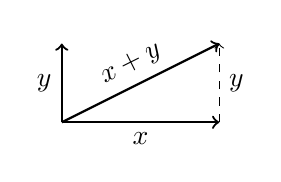
\begin{tikzpicture}
    \draw[thick,->] (0,0) -- (2,0) node[pos=0.5, below] {$x$};
    \draw[thick,->] (0,0) -- (0,1) node[pos=0.5, left] {$y$};
    \draw[thick,->] (0,0) -- (2,1) node[pos=0.5, rotate=26.57, above] {$x+y$};
    \draw[dashed,->] (2,0) -- (2,1) node[pos=0.5, right] {$y$};
\end{tikzpicture}
    \caption{Illustration of the Pythagorean Theorem in the plane}
    \label{fig:sec3-1-ex2}
\end{figure}

\end{exercise}
\begin{proof}
We have
\begin{align*}
    \norm{x+y}^2
    =& \brackets{x+y, x+y}\\
    =& \brackets{x, x+y} + \brackets{y, x+y}\\
    =& \overline{\brackets{x+y, x}} + \overline{\brackets{x+y,y}}\\
    =& \overline{\brackets{x, x} + \brackets{y, x}} + \overline{\brackets{x,y} + \brackets{y,y}}\\
    =& \brackets{x, x} + \brackets{y,y}\\
    =& \norm{x}^2 +\norm{y}^2,
\end{align*}
as required.

Extending the formula to $m$ mutually orthogonal vectors would give us
\begin{align*}
    \norm{x_1+\dots+x_m}^2
    = \norm{x_1}^2 + \dots + \norm{x_m}^2.
\end{align*}
\end{proof}

\begin{exercise}{3}
If $X$ in exercise 2 is real, show that, conversely the given relation implies that $x\perp y$. 
Show that this may not hold if $X$ is complex. Give examples.
\end{exercise}
\begin{proof}
Suppose then that $X$ is real and that $\norm{x+y}^2 = \norm{x}^2 + \norm{y}^2$.
We have
\begin{align*}
    \norm{x}^2 + \norm{y}^2
    =& \norm{x+y}^2\\
    =& \brackets{x+y, x+y}\\
    =& \brackets{x, x+y} + \brackets{y, x+y}\\
    =& \brackets{x+y, x} + \brackets{x+y,y}\\
    =& \brackets{x, x} + \brackets{y, x} 
    + \brackets{x,y} + \brackets{y,y}\\
    =& \norm{x}^2 + \norm{y}^2 + 2\brackets{x,y}.
\end{align*}
Thus $2\brackets{x,y}=0$, so that $x\perp y$.

Now consider $1,i\in\C$. 
We have $\norm{1+i}^2 = 1^2 + 1^2 = \norm{1}^2 + \norm{i}^2$, however, $\brackets{1,i} = -i\brackets{1,1} = -i$, so that they are not orthogonal.
\end{proof}

\begin{exercise}{6}
Let $x\neq 0$ and $y\neq 0$.
\begin{enumerate}
    \item If $x\perp y$, show that $\set{x,y}$ is a linearly independent set.
    \item Extend the result to mutually orthogonal nonzero vectors $x_1,\dots, x_m$.
\end{enumerate}
\end{exercise}
\begin{proof}
\begin{enumerate}
    \item We will prove this by contrapositive.
    Suppose $x$ and $y$ are not linearly independent, so that $x=ay$ for some scalar $a$.
    We then have
    \begin{align*}
        \brackets{x,y}
        = \brackets{ay, y} 
        = a\brackets{y,y} 
        \neq 0,
    \end{align*}
    so that $x$ is not orthogonal to $y$.
    \item There are many ways in which we can extend this idea to many vectors.
    One could be to force $x_i$ to be orthogonal to any linear combination of the rest of the vectors.
\end{enumerate}
\end{proof}

\begin{exercise}{7}
If in an inner product space $\brackets{x,u} = \brackets{x,v}$ for all $x$, show that $u=v$.
\end{exercise}
\begin{proof}
Consider $x=u-v$.
We have
\begin{align*}
    &\brackets{u-v, u} = \brackets{u-v, v} &&\iff\\
    &\brackets{u-v, u} - \brackets{u-v, v} &&\iff\\
    &\overline{\brackets{u, u-v}} - \overline{\brackets{v, u-v}} = 0 &&\iff\\
    &\overline{\brackets{u-v,u-v}} = 0 &&\iff\\
    &\norm{u-v} = 0.
\end{align*}
Norms have the property that $\norm{x} = 0$ if and only if $x=0$, thus $u-v=0$ and $u=v$, as required.
\end{proof}

\begin{exercise}{9}
Prove that
\begin{align*}
    \text{Re}\brackets{x,y} = 1/4[\norm{x+y}^2-\norm{x-y}^2];\quad \text{Im}\brackets{x,y} = 1/4[\norm{x+iy}^2-\norm{x-iy}^2]
\end{align*}
\end{exercise}
\begin{proof}
($\text{Re}\brackets{x,y}$)
We have 
\begin{align*}
    \norm{x+y}^2 = \norm{x}^2 +\norm{y}^2 + \overline{\brackets{y,x}} + \overline{\brackets{x,y}},
\end{align*}
and
\begin{align*}
    \norm{x-y}^2 = 
    \norm{x}^2 +\norm{y}^2 -\overline{\brackets{y,x}} - \overline{\brackets{x,y}}.
\end{align*}
So that
\begin{align*}
    1/4[\norm{x+y}^2 -\norm{x-y}^2]
    =& 1/4[2\overline{\brackets{y,x}} + 2\overline{\brackets{x,y}}]\\
    =& 1/2[2\text{Re}\brackets{x,y}],
\end{align*}
as required.
Where the last equality follows from Axler 4.5, for example.

($\text{Im}\brackets{x,y}$)
We have
\begin{align*}
    \norm{x+iy}^2
    =& \brackets{x+iy, x+iy}\\
    =& \brackets{x,x+iy} + i\brackets{y,x+iy}\\
    =& \overline{\brackets{x+iy,x}} +i\overline{\brackets{x+iy,y}}\\
    =& \overline{\brackets{x,x} + i\brackets{y,x}} + i[\overline{\brackets{x,y} + i\brackets{y,y}}]\\
    =& \norm{x}^2 + \norm{y}^2 - i\overline{\brackets{y,x}} + i\overline{\brackets{x,y}},
\end{align*}
and
\begin{align*}
    \norm{x-iy}^2
    =& \brackets{x-iy, x-iy}\\
    =& \brackets{x,x-iy} - i\brackets{y,x-iy}\\
    =& \overline{\brackets{x-iy,x}} -i\overline{\brackets{x-iy,y}}\\
    =& \overline{\brackets{x,x} - i\brackets{y,x}} - i[\overline{\brackets{x,y} - i\brackets{y,y}}]\\
    =& \norm{x}^2 + \norm{y}^2 + i\overline{\brackets{y,x}} - i\overline{\brackets{x,y}}.
\end{align*}
We use these two together to obtain
\begin{align*}
    1/4[\norm{x+iy}^2-\norm{x-iy}^2]
    =& 1/4[i2\overline{\brackets{x,y}} -i2\overline{\brackets{y,x}}]\\
    =& -i/2[\brackets{x,y}-\overline{\brackets{x,y}}\\
    =& -i/2[2i\text{Im}(x,y)] = \text{Im}\brackets{x,y},
\end{align*}
as required.
\end{proof}

\begin{exercise}{10}
Let $x$ and $y$ denote complex numbers.
Show that $\brackets{x,y} = x\bar{y}$ defines an inner product, which yields the usual metric on the complex plane.
Under what condition do we have orthogonality?
\end{exercise}
\begin{proof}
(IP1)
Suppose $z\in\C$.
We have 
\begin{align*}
    \brackets{(x+y),z}
    = (x+y)\bar{z}
    = x\bar{z} + y\bar{z}
    = \brackets{x,z} + \brackets{y,z}.
\end{align*}

(IP2)
Suppose $a\in\C$.
We have
\begin{align*}
    \brackets{ax,y}
    = ax\bar{y}
    = a\brackets{x,y}.
\end{align*}

(IP3)
We have
\begin{align*}
    \overline{\brackets{x,y}}
    = \overline{x\bar{y}}
    = \bar{x}\overline{\bar{y}}
    = \bar{x}y
    = y\bar{x}
    = \brackets{y,x}.
\end{align*}

(IP4)
We have
\begin{align*}
    \brackets{x,x}
    = x\bar{x}
    = \absoluteValue{x}^2 \geq 0,
\end{align*}
with equality if and only if $x=0$.

(Orthogonality)
Write $x=a+bi$ and $y=c+di$.
We then have
\begin{align*}
    0
    =& \brackets{x,y} && \iff\\
    =& (a+bi)\overline{(c+di)} &&\iff\\
    =& ac - aci + cbi - bdi^2 &&\iff\\
    =& (ac+bd) + (cb-ad)i.
\end{align*}
So orthogonolity holds when $ac=-bd$ and $cb=ad$.
\end{proof}

\begin{exercise}{11}
Let $X$ be the vector space of all ordered pairs of complex numbers.
Can we obtain the norm defined on $X$ by $\norm{x} =\absoluteValue{x_1}+\absoluteValue{x_2}$ from an inner product?
\end{exercise}
\begin{proof}
No, consider $x =(1,1), y=(1,-1) \in\C$.
We have
\begin{align*}
    &\norm{x+y}^2 = \absoluteValue{2}^2\\
    &\norm{x-y}^2 = \absoluteValue{2}^2\\
    &\norm{x}^2 = \sqrt{1^2+1^2}^2\\
    &\norm{y}^2 = \sqrt{1^2+(-1)^2}^2.
\end{align*}
Thus the parallelogram equality
\begin{align*}
    \norm{x+y}^2 + \norm{x-y}^2 = 
    2[\norm{x}^2 + \norm{y}^2]
\end{align*}
does not hold, and thus the norm cannot be obtained by an inner product.
\end{proof}

\begin{exercise}{15}
If $X$ is a finite dimensional vector space and $(e_j)$ is a basis for $X$, show that an inner product on $X$ is completely determined by its values $\gamma_{jk}=\brackets{e_j,e_k}$.
Can we choose such scalars $\gamma_{jk}$ in a completely arbitrary fashion?
\end{exercise}
\begin{proof}
Take any $x,x'\in X$.
We have 
\begin{align*}
    \brackets{x,x'}
    =& \brackets{a_1e_1+\dots+a_ne_n, a_1'e_1+\dots+a_n'e_n}\\
    =& \brackets{a_1e_1,a_1'e_1+\dots+a_n'e_n} + \dots + \brackets{a_ne_n,a_1'e_1+\dots+a_n'e_n}\\
    =& \overline{\brackets{a_1'e_1+\dots+a_n'e_n, a_1e_1}} + \dots + \overline{\brackets{a_1'e_1+\dots+a_n'e_n, a_ne_n}}\\
    =& \overline{\brackets{a_1'e_1, a_1e_1}} + \dots \overline{\brackets{a_n'e_n, a_1e_1}} + \dots + \overline{\brackets{a_1'e_1, a_ne_n}} + \dots +
    \overline{\brackets{a_n'e_n, a_ne_n}}\\
    =& \overline{a_1'\bar{a_1}\brackets{e_1, e_1}} + \dots \overline{a_n'\bar{a_1}\brackets{e_n, e_1}} + \dots + \overline{a_1'\bar{a_n}\brackets{e_1, e_n}} + \dots +
    \overline{a_n'\bar{a_n}\brackets{e_n, e_n}}\\
    =& \overline{a_1'\bar{a_1}\gamma_{1,1}} + \dots \overline{a_n'\bar{a_1}\gamma_{n,1}} + \dots + \overline{a_1'\bar{a_n}\gamma_{1,n}} + \dots +
    \overline{a_n'\bar{a_n}\gamma_{n,n}}.
\end{align*}
so that the value of the inner product is completely determined by $\gamma_{j,k}$.

For $\gamma_{j,k}$ to be valid, we need $\gamma_{j,j}>0$ and $\gamma_{j,k}=\overline{\gamma_{k,j}}$, which implies that the matrix representing the inner product is self-adjoint.
\end{proof}
